% layout and global options
\documentclass
[
  fontsize = 11pt,
  parskip  = half-,
  BCOR     = 0pt,
  DIV      = 11,
  draft,
  ngerman,
  dvipsnames
]
{scrartcl}

% default packages
\usepackage[utf8]{inputenc}
\usepackage[T1]{fontenc}
\usepackage{babel}
\usepackage{lmodern}
% extra packages
\usepackage{amsmath}
\usepackage{amssymb}
\usepackage{enumerate}
\usepackage{eurosym}
\usepackage{graphicx}
\usepackage{ifthen}
\usepackage{siunitx}
\usepackage{tikz}

% enable calculations in TikZ
\usetikzlibrary{calc}

% use comma as decimal separator
\sisetup{locale=DE, group-minimum-digits=4}

% no headers no footers
\pagestyle{empty}

% ------------------------------------------------------------------------------
\begin{document}
% ------------------------------------------------------------------------------

\enlargethispage{1\baselineskip}%

% -------------------------
\section*{Potenzfunktionen}
% -------------------------
\begin{equation*}
  f(x)=a\cdot x^n
\end{equation*}

% ---------------------------------
\paragraph{Typ \glqq ungerade\grqq}\leavevmode\par
% ---------------------------------
%<OCTAVE>
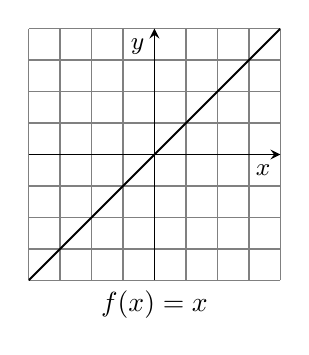
\begin{tikzpicture}[scale=0.800]
  % grid
  \draw[draw=black!50!white] (-2.000, -2.000) grid[step=0.5] (2.000, 2.000);
  % x-axis
  \draw[line width=0.6pt, ->, >=stealth] (-2.000, 0) -- (2.000, 0) node[below left] {\small$x$};
  % y-axis
  \draw[line width=0.6pt, ->, >=stealth] (0, -2.000) -- (0, 2.000) node[below left] {\small$y$};
  % function: f(x)=x
  \begin{scope}[line width=0.7pt]
    \clip (-2.000, -2.000) rectangle (2.000, 2.000);
    \draw plot[smooth] coordinates
    {
      ( -2.000,  -2.000) ( -1.900,  -1.900) ( -1.800,  -1.800)
      ( -1.700,  -1.700) ( -1.600,  -1.600) ( -1.500,  -1.500)
      ( -1.400,  -1.400) ( -1.300,  -1.300) ( -1.200,  -1.200)
      ( -1.100,  -1.100) ( -1.000,  -1.000) ( -0.900,  -0.900)
      ( -0.800,  -0.800) ( -0.700,  -0.700) ( -0.600,  -0.600)
      ( -0.500,  -0.500) ( -0.400,  -0.400) ( -0.300,  -0.300)
      ( -0.200,  -0.200) ( -0.100,  -0.100) (  0.000,   0.000)
      (  0.100,   0.100) (  0.200,   0.200) (  0.300,   0.300)
      (  0.400,   0.400) (  0.500,   0.500) (  0.600,   0.600)
      (  0.700,   0.700) (  0.800,   0.800) (  0.900,   0.900)
      (  1.000,   1.000) (  1.100,   1.100) (  1.200,   1.200)
      (  1.300,   1.300) (  1.400,   1.400) (  1.500,   1.500)
      (  1.600,   1.600) (  1.700,   1.700) (  1.800,   1.800)
      (  1.900,   1.900) (  2.000,   2.000)
    };
  \end{scope}
  \node[below] at (0, -2) {$f(x)=x$};
\end{tikzpicture}
%</OCTAVE>
%mypolyplot([1 0], -2, 2, -2, 2, 0.1, 0.8)
\hfill
%<OCTAVE>
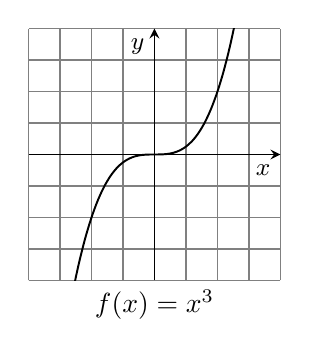
\begin{tikzpicture}[scale=0.800]
  % grid
  \draw[draw=black!50!white] (-2.000, -2.000) grid[step=0.5] (2.000, 2.000);
  % x-axis
  \draw[line width=0.6pt, ->, >=stealth] (-2.000, 0) -- (2.000, 0) node[below left] {\small$x$};
  % y-axis
  \draw[line width=0.6pt, ->, >=stealth] (0, -2.000) -- (0, 2.000) node[below left] {\small$y$};
  % function: f(x)=x^{3}
  \begin{scope}[line width=0.7pt]
    \clip (-2.000, -2.000) rectangle (2.000, 2.000);
    \draw plot[smooth] coordinates
    {
      ( -2.000,  -5.000) ( -1.900,  -5.000) ( -1.800,  -5.000)
      ( -1.700,  -4.913) ( -1.600,  -4.096) ( -1.500,  -3.375)
      ( -1.400,  -2.744) ( -1.300,  -2.197) ( -1.200,  -1.728)
      ( -1.100,  -1.331) ( -1.000,  -1.000) ( -0.900,  -0.729)
      ( -0.800,  -0.512) ( -0.700,  -0.343) ( -0.600,  -0.216)
      ( -0.500,  -0.125) ( -0.400,  -0.064) ( -0.300,  -0.027)
      ( -0.200,  -0.008) ( -0.100,  -0.001) (  0.000,   0.000)
      (  0.100,   0.001) (  0.200,   0.008) (  0.300,   0.027)
      (  0.400,   0.064) (  0.500,   0.125) (  0.600,   0.216)
      (  0.700,   0.343) (  0.800,   0.512) (  0.900,   0.729)
      (  1.000,   1.000) (  1.100,   1.331) (  1.200,   1.728)
      (  1.300,   2.197) (  1.400,   2.744) (  1.500,   3.375)
      (  1.600,   4.096) (  1.700,   4.913) (  1.800,   5.000)
      (  1.900,   5.000) (  2.000,   5.000)
    };
  \end{scope}
  \node[below] at (0, -2) {$f(x)=x^3$};
\end{tikzpicture}
%</OCTAVE>
%mypolyplot([1 0 0 0], -2, 2, -2, 2, 0.1, 0.8)
\hfill
%<OCTAVE>
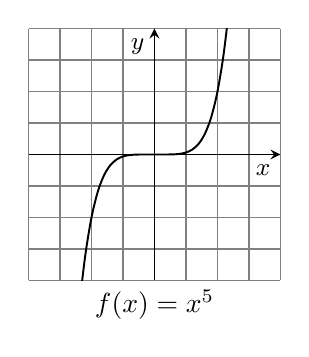
\begin{tikzpicture}[scale=0.800]
  % grid
  \draw[draw=black!50!white] (-2.000, -2.000) grid[step=0.5] (2.000, 2.000);
  % x-axis
  \draw[line width=0.6pt, ->, >=stealth] (-2.000, 0) -- (2.000, 0) node[below left] {\small$x$};
  % y-axis
  \draw[line width=0.6pt, ->, >=stealth] (0, -2.000) -- (0, 2.000) node[below left] {\small$y$};
  % function: f(x)=x^{5}
  \begin{scope}[line width=0.7pt]
    \clip (-2.000, -2.000) rectangle (2.000, 2.000);
    \draw plot[smooth] coordinates
    {
      ( -2.000,  -5.000) ( -1.900,  -5.000) ( -1.800,  -5.000)
      ( -1.700,  -5.000) ( -1.600,  -5.000) ( -1.500,  -5.000)
      ( -1.400,  -5.000) ( -1.300,  -3.713) ( -1.200,  -2.488)
      ( -1.100,  -1.611) ( -1.000,  -1.000) ( -0.900,  -0.590)
      ( -0.800,  -0.328) ( -0.700,  -0.168) ( -0.600,  -0.078)
      ( -0.500,  -0.031) ( -0.400,  -0.010) ( -0.300,  -0.002)
      ( -0.200,  -0.000) ( -0.100,  -0.000) (  0.000,   0.000)
      (  0.100,   0.000) (  0.200,   0.000) (  0.300,   0.002)
      (  0.400,   0.010) (  0.500,   0.031) (  0.600,   0.078)
      (  0.700,   0.168) (  0.800,   0.328) (  0.900,   0.590)
      (  1.000,   1.000) (  1.100,   1.611) (  1.200,   2.488)
      (  1.300,   3.713) (  1.400,   5.000) (  1.500,   5.000)
      (  1.600,   5.000) (  1.700,   5.000) (  1.800,   5.000)
      (  1.900,   5.000) (  2.000,   5.000)
    };
  \end{scope}
  \node[below] at (0, -2) {$f(x)=x^5$};
\end{tikzpicture}
%</OCTAVE>
%mypolyplot([1 0 0 0 0 0], -2, 2, -2, 2, 0.1, 0.8)
\hfill
%<OCTAVE>
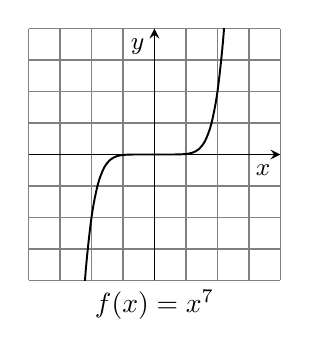
\begin{tikzpicture}[scale=0.800]
  % grid
  \draw[draw=black!50!white] (-2.000, -2.000) grid[step=0.5] (2.000, 2.000);
  % x-axis
  \draw[line width=0.6pt, ->, >=stealth] (-2.000, 0) -- (2.000, 0) node[below left] {\small$x$};
  % y-axis
  \draw[line width=0.6pt, ->, >=stealth] (0, -2.000) -- (0, 2.000) node[below left] {\small$y$};
  % function: f(x)=x^{7}
  \begin{scope}[line width=0.7pt]
    \clip (-2.000, -2.000) rectangle (2.000, 2.000);
    \draw plot[smooth] coordinates
    {
      ( -2.000,  -5.000) ( -1.900,  -5.000) ( -1.800,  -5.000)
      ( -1.700,  -5.000) ( -1.600,  -5.000) ( -1.500,  -5.000)
      ( -1.400,  -5.000) ( -1.300,  -5.000) ( -1.200,  -3.583)
      ( -1.100,  -1.949) ( -1.000,  -1.000) ( -0.900,  -0.478)
      ( -0.800,  -0.210) ( -0.700,  -0.082) ( -0.600,  -0.028)
      ( -0.500,  -0.008) ( -0.400,  -0.002) ( -0.300,  -0.000)
      ( -0.200,  -0.000) ( -0.100,  -0.000) (  0.000,   0.000)
      (  0.100,   0.000) (  0.200,   0.000) (  0.300,   0.000)
      (  0.400,   0.002) (  0.500,   0.008) (  0.600,   0.028)
      (  0.700,   0.082) (  0.800,   0.210) (  0.900,   0.478)
      (  1.000,   1.000) (  1.100,   1.949) (  1.200,   3.583)
      (  1.300,   5.000) (  1.400,   5.000) (  1.500,   5.000)
      (  1.600,   5.000) (  1.700,   5.000) (  1.800,   5.000)
      (  1.900,   5.000) (  2.000,   5.000)
    };
  \end{scope}
  \node[below] at (0, -2) {$f(x)=x^7$};
\end{tikzpicture}
%</OCTAVE>
%mypolyplot([1 0 0 0 0 0 0 0], -2, 2, -2, 2, 0.1, 0.8)

% -------------------------------
\paragraph{Typ \glqq gerade\grqq}\leavevmode\par
% -------------------------------
%<OCTAVE>
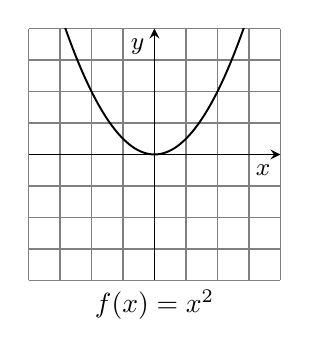
\begin{tikzpicture}[scale=0.800]
  % grid
  \draw[draw=black!50!white] (-2.000, -2.000) grid[step=0.5] (2.000, 2.000);
  % x-axis
  \draw[line width=0.6pt, ->, >=stealth] (-2.000, 0) -- (2.000, 0) node[below left] {\small$x$};
  % y-axis
  \draw[line width=0.6pt, ->, >=stealth] (0, -2.000) -- (0, 2.000) node[below left] {\small$y$};
  % function: f(x)=x^{2}
  \begin{scope}[line width=0.7pt]
    \clip (-2.000, -2.000) rectangle (2.000, 2.000);
    \draw plot[smooth] coordinates
    {
      ( -2.000,   4.000) ( -1.900,   3.610) ( -1.800,   3.240)
      ( -1.700,   2.890) ( -1.600,   2.560) ( -1.500,   2.250)
      ( -1.400,   1.960) ( -1.300,   1.690) ( -1.200,   1.440)
      ( -1.100,   1.210) ( -1.000,   1.000) ( -0.900,   0.810)
      ( -0.800,   0.640) ( -0.700,   0.490) ( -0.600,   0.360)
      ( -0.500,   0.250) ( -0.400,   0.160) ( -0.300,   0.090)
      ( -0.200,   0.040) ( -0.100,   0.010) (  0.000,   0.000)
      (  0.100,   0.010) (  0.200,   0.040) (  0.300,   0.090)
      (  0.400,   0.160) (  0.500,   0.250) (  0.600,   0.360)
      (  0.700,   0.490) (  0.800,   0.640) (  0.900,   0.810)
      (  1.000,   1.000) (  1.100,   1.210) (  1.200,   1.440)
      (  1.300,   1.690) (  1.400,   1.960) (  1.500,   2.250)
      (  1.600,   2.560) (  1.700,   2.890) (  1.800,   3.240)
      (  1.900,   3.610) (  2.000,   4.000)
    };
  \end{scope}
  \node[below] at (0, -2) {$f(x)=x^2$};
\end{tikzpicture}
%</OCTAVE>
%mypolyplot([1 0 0], -2, 2, -2, 2, 0.1, 0.8)
\hfill
%<OCTAVE>
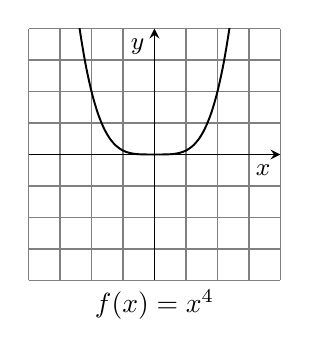
\begin{tikzpicture}[scale=0.800]
  % grid
  \draw[draw=black!50!white] (-2.000, -2.000) grid[step=0.5] (2.000, 2.000);
  % x-axis
  \draw[line width=0.6pt, ->, >=stealth] (-2.000, 0) -- (2.000, 0) node[below left] {\small$x$};
  % y-axis
  \draw[line width=0.6pt, ->, >=stealth] (0, -2.000) -- (0, 2.000) node[below left] {\small$y$};
  % function: f(x)=x^{4}
  \begin{scope}[line width=0.7pt]
    \clip (-2.000, -2.000) rectangle (2.000, 2.000);
    \draw plot[smooth] coordinates
    {
      ( -2.000,   5.000) ( -1.900,   5.000) ( -1.800,   5.000)
      ( -1.700,   5.000) ( -1.600,   5.000) ( -1.500,   5.000)
      ( -1.400,   3.842) ( -1.300,   2.856) ( -1.200,   2.074)
      ( -1.100,   1.464) ( -1.000,   1.000) ( -0.900,   0.656)
      ( -0.800,   0.410) ( -0.700,   0.240) ( -0.600,   0.130)
      ( -0.500,   0.062) ( -0.400,   0.026) ( -0.300,   0.008)
      ( -0.200,   0.002) ( -0.100,   0.000) (  0.000,   0.000)
      (  0.100,   0.000) (  0.200,   0.002) (  0.300,   0.008)
      (  0.400,   0.026) (  0.500,   0.062) (  0.600,   0.130)
      (  0.700,   0.240) (  0.800,   0.410) (  0.900,   0.656)
      (  1.000,   1.000) (  1.100,   1.464) (  1.200,   2.074)
      (  1.300,   2.856) (  1.400,   3.842) (  1.500,   5.000)
      (  1.600,   5.000) (  1.700,   5.000) (  1.800,   5.000)
      (  1.900,   5.000) (  2.000,   5.000)
    };
  \end{scope}
  \node[below] at (0, -2) {$f(x)=x^4$};
\end{tikzpicture}
%</OCTAVE>
%mypolyplot([1 0 0 0 0], -2, 2, -2, 2, 0.1, 0.8)
\hfill
%<OCTAVE>
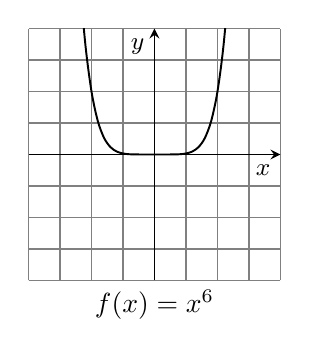
\begin{tikzpicture}[scale=0.800]
  % grid
  \draw[draw=black!50!white] (-2.000, -2.000) grid[step=0.5] (2.000, 2.000);
  % x-axis
  \draw[line width=0.6pt, ->, >=stealth] (-2.000, 0) -- (2.000, 0) node[below left] {\small$x$};
  % y-axis
  \draw[line width=0.6pt, ->, >=stealth] (0, -2.000) -- (0, 2.000) node[below left] {\small$y$};
  % function: f(x)=x^{6}
  \begin{scope}[line width=0.7pt]
    \clip (-2.000, -2.000) rectangle (2.000, 2.000);
    \draw plot[smooth] coordinates
    {
      ( -2.000,   5.000) ( -1.900,   5.000) ( -1.800,   5.000)
      ( -1.700,   5.000) ( -1.600,   5.000) ( -1.500,   5.000)
      ( -1.400,   5.000) ( -1.300,   4.827) ( -1.200,   2.986)
      ( -1.100,   1.772) ( -1.000,   1.000) ( -0.900,   0.531)
      ( -0.800,   0.262) ( -0.700,   0.118) ( -0.600,   0.047)
      ( -0.500,   0.016) ( -0.400,   0.004) ( -0.300,   0.001)
      ( -0.200,   0.000) ( -0.100,   0.000) (  0.000,   0.000)
      (  0.100,   0.000) (  0.200,   0.000) (  0.300,   0.001)
      (  0.400,   0.004) (  0.500,   0.016) (  0.600,   0.047)
      (  0.700,   0.118) (  0.800,   0.262) (  0.900,   0.531)
      (  1.000,   1.000) (  1.100,   1.772) (  1.200,   2.986)
      (  1.300,   4.827) (  1.400,   5.000) (  1.500,   5.000)
      (  1.600,   5.000) (  1.700,   5.000) (  1.800,   5.000)
      (  1.900,   5.000) (  2.000,   5.000)
    };
  \end{scope}
  \node[below] at (0, -2) {$f(x)=x^6$};
\end{tikzpicture}
%</OCTAVE>
%mypolyplot([1 0 0 0 0 0 0], -2, 2, -2, 2, 0.1, 0.8)
\hfill
%<OCTAVE>
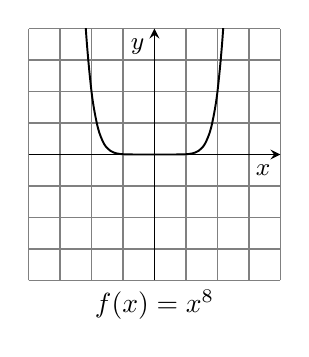
\begin{tikzpicture}[scale=0.800]
  % grid
  \draw[draw=black!50!white] (-2.000, -2.000) grid[step=0.5] (2.000, 2.000);
  % x-axis
  \draw[line width=0.6pt, ->, >=stealth] (-2.000, 0) -- (2.000, 0) node[below left] {\small$x$};
  % y-axis
  \draw[line width=0.6pt, ->, >=stealth] (0, -2.000) -- (0, 2.000) node[below left] {\small$y$};
  % function: f(x)=x^{8}
  \begin{scope}[line width=0.7pt]
    \clip (-2.000, -2.000) rectangle (2.000, 2.000);
    \draw plot[smooth] coordinates
    {
      ( -2.000,   5.000) ( -1.900,   5.000) ( -1.800,   5.000)
      ( -1.700,   5.000) ( -1.600,   5.000) ( -1.500,   5.000)
      ( -1.400,   5.000) ( -1.300,   5.000) ( -1.200,   4.300)
      ( -1.100,   2.144) ( -1.000,   1.000) ( -0.900,   0.430)
      ( -0.800,   0.168) ( -0.700,   0.058) ( -0.600,   0.017)
      ( -0.500,   0.004) ( -0.400,   0.001) ( -0.300,   0.000)
      ( -0.200,   0.000) ( -0.100,   0.000) (  0.000,   0.000)
      (  0.100,   0.000) (  0.200,   0.000) (  0.300,   0.000)
      (  0.400,   0.001) (  0.500,   0.004) (  0.600,   0.017)
      (  0.700,   0.058) (  0.800,   0.168) (  0.900,   0.430)
      (  1.000,   1.000) (  1.100,   2.144) (  1.200,   4.300)
      (  1.300,   5.000) (  1.400,   5.000) (  1.500,   5.000)
      (  1.600,   5.000) (  1.700,   5.000) (  1.800,   5.000)
      (  1.900,   5.000) (  2.000,   5.000)
    };
  \end{scope}
  \node[below] at (0, -2) {$f(x)=x^8$};
\end{tikzpicture}
%</OCTAVE>
%mypolyplot([1 0 0 0 0 0 0 0 0], -2, 2, -2, 2, 0.1, 0.8)

% --------------------
\paragraph{Spiegelung}
% --------------------
Mit $a=-1$ ergibt sich eine Spiegelung an der
$x$-Achse:\par

%<OCTAVE>
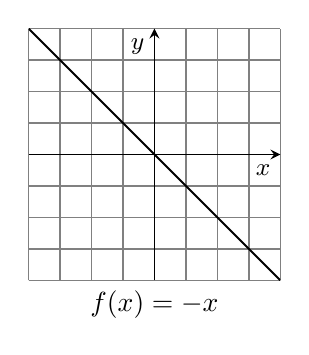
\begin{tikzpicture}[scale=0.800]
  % grid
  \draw[draw=black!50!white] (-2.000, -2.000) grid[step=0.5] (2.000, 2.000);
  % x-axis
  \draw[line width=0.6pt, ->, >=stealth] (-2.000, 0) -- (2.000, 0) node[below left] {\small$x$};
  % y-axis
  \draw[line width=0.6pt, ->, >=stealth] (0, -2.000) -- (0, 2.000) node[below left] {\small$y$};
  % function: f(x)=-x
  \begin{scope}[line width=0.7pt]
    \clip (-2.000, -2.000) rectangle (2.000, 2.000);
    \draw plot[smooth] coordinates
    {
      ( -2.000,   2.000) ( -1.900,   1.900) ( -1.800,   1.800)
      ( -1.700,   1.700) ( -1.600,   1.600) ( -1.500,   1.500)
      ( -1.400,   1.400) ( -1.300,   1.300) ( -1.200,   1.200)
      ( -1.100,   1.100) ( -1.000,   1.000) ( -0.900,   0.900)
      ( -0.800,   0.800) ( -0.700,   0.700) ( -0.600,   0.600)
      ( -0.500,   0.500) ( -0.400,   0.400) ( -0.300,   0.300)
      ( -0.200,   0.200) ( -0.100,   0.100) (  0.000,   0.000)
      (  0.100,  -0.100) (  0.200,  -0.200) (  0.300,  -0.300)
      (  0.400,  -0.400) (  0.500,  -0.500) (  0.600,  -0.600)
      (  0.700,  -0.700) (  0.800,  -0.800) (  0.900,  -0.900)
      (  1.000,  -1.000) (  1.100,  -1.100) (  1.200,  -1.200)
      (  1.300,  -1.300) (  1.400,  -1.400) (  1.500,  -1.500)
      (  1.600,  -1.600) (  1.700,  -1.700) (  1.800,  -1.800)
      (  1.900,  -1.900) (  2.000,  -2.000)
    };
  \end{scope}
  \node[below] at (0, -2) {$f(x)=-x$};
\end{tikzpicture}
%</OCTAVE>
%mypolyplot([-1 0], -2, 2, -2, 2, 0.1, 0.8)
\hfill
%<OCTAVE>
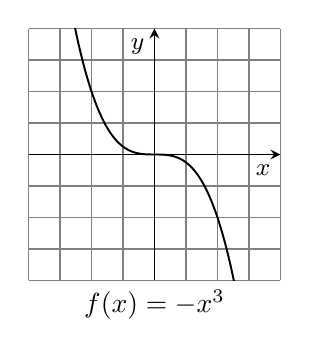
\begin{tikzpicture}[scale=0.800]
  % grid
  \draw[draw=black!50!white] (-2.000, -2.000) grid[step=0.5] (2.000, 2.000);
  % x-axis
  \draw[line width=0.6pt, ->, >=stealth] (-2.000, 0) -- (2.000, 0) node[below left] {\small$x$};
  % y-axis
  \draw[line width=0.6pt, ->, >=stealth] (0, -2.000) -- (0, 2.000) node[below left] {\small$y$};
  % function: f(x)=-x^{3}
  \begin{scope}[line width=0.7pt]
    \clip (-2.000, -2.000) rectangle (2.000, 2.000);
    \draw plot[smooth] coordinates
    {
      ( -2.000,   5.000) ( -1.900,   5.000) ( -1.800,   5.000)
      ( -1.700,   4.913) ( -1.600,   4.096) ( -1.500,   3.375)
      ( -1.400,   2.744) ( -1.300,   2.197) ( -1.200,   1.728)
      ( -1.100,   1.331) ( -1.000,   1.000) ( -0.900,   0.729)
      ( -0.800,   0.512) ( -0.700,   0.343) ( -0.600,   0.216)
      ( -0.500,   0.125) ( -0.400,   0.064) ( -0.300,   0.027)
      ( -0.200,   0.008) ( -0.100,   0.001) (  0.000,   0.000)
      (  0.100,  -0.001) (  0.200,  -0.008) (  0.300,  -0.027)
      (  0.400,  -0.064) (  0.500,  -0.125) (  0.600,  -0.216)
      (  0.700,  -0.343) (  0.800,  -0.512) (  0.900,  -0.729)
      (  1.000,  -1.000) (  1.100,  -1.331) (  1.200,  -1.728)
      (  1.300,  -2.197) (  1.400,  -2.744) (  1.500,  -3.375)
      (  1.600,  -4.096) (  1.700,  -4.913) (  1.800,  -5.000)
      (  1.900,  -5.000) (  2.000,  -5.000)
    };
  \end{scope}
  \node[below] at (0, -2) {$f(x)=-x^3$};
\end{tikzpicture}
%</OCTAVE>
%mypolyplot([-1 0 0 0], -2, 2, -2, 2, 0.1, 0.8)
\hfill
%<OCTAVE>
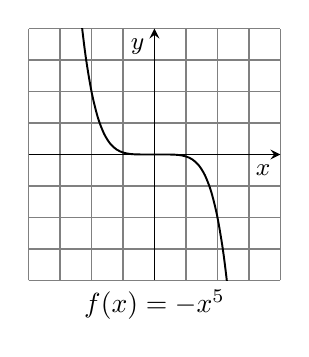
\begin{tikzpicture}[scale=0.800]
  % grid
  \draw[draw=black!50!white] (-2.000, -2.000) grid[step=0.5] (2.000, 2.000);
  % x-axis
  \draw[line width=0.6pt, ->, >=stealth] (-2.000, 0) -- (2.000, 0) node[below left] {\small$x$};
  % y-axis
  \draw[line width=0.6pt, ->, >=stealth] (0, -2.000) -- (0, 2.000) node[below left] {\small$y$};
  % function: f(x)=-x^{5}
  \begin{scope}[line width=0.7pt]
    \clip (-2.000, -2.000) rectangle (2.000, 2.000);
    \draw plot[smooth] coordinates
    {
      ( -2.000,   5.000) ( -1.900,   5.000) ( -1.800,   5.000)
      ( -1.700,   5.000) ( -1.600,   5.000) ( -1.500,   5.000)
      ( -1.400,   5.000) ( -1.300,   3.713) ( -1.200,   2.488)
      ( -1.100,   1.611) ( -1.000,   1.000) ( -0.900,   0.590)
      ( -0.800,   0.328) ( -0.700,   0.168) ( -0.600,   0.078)
      ( -0.500,   0.031) ( -0.400,   0.010) ( -0.300,   0.002)
      ( -0.200,   0.000) ( -0.100,   0.000) (  0.000,   0.000)
      (  0.100,  -0.000) (  0.200,  -0.000) (  0.300,  -0.002)
      (  0.400,  -0.010) (  0.500,  -0.031) (  0.600,  -0.078)
      (  0.700,  -0.168) (  0.800,  -0.328) (  0.900,  -0.590)
      (  1.000,  -1.000) (  1.100,  -1.611) (  1.200,  -2.488)
      (  1.300,  -3.713) (  1.400,  -5.000) (  1.500,  -5.000)
      (  1.600,  -5.000) (  1.700,  -5.000) (  1.800,  -5.000)
      (  1.900,  -5.000) (  2.000,  -5.000)
    };
  \end{scope}
  \node[below] at (0, -2) {$f(x)=-x^5$};
\end{tikzpicture}
%</OCTAVE>
%mypolyplot([-1 0 0 0 0 0], -2, 2, -2, 2, 0.1, 0.8)
\hfill
%<OCTAVE>
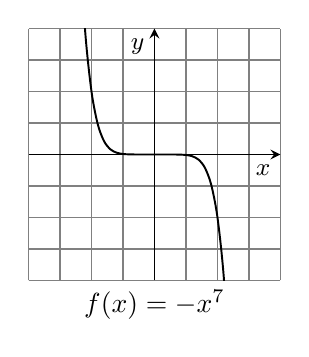
\begin{tikzpicture}[scale=0.800]
  % grid
  \draw[draw=black!50!white] (-2.000, -2.000) grid[step=0.5] (2.000, 2.000);
  % x-axis
  \draw[line width=0.6pt, ->, >=stealth] (-2.000, 0) -- (2.000, 0) node[below left] {\small$x$};
  % y-axis
  \draw[line width=0.6pt, ->, >=stealth] (0, -2.000) -- (0, 2.000) node[below left] {\small$y$};
  % function: f(x)=-x^{7}
  \begin{scope}[line width=0.7pt]
    \clip (-2.000, -2.000) rectangle (2.000, 2.000);
    \draw plot[smooth] coordinates
    {
      ( -2.000,   5.000) ( -1.900,   5.000) ( -1.800,   5.000)
      ( -1.700,   5.000) ( -1.600,   5.000) ( -1.500,   5.000)
      ( -1.400,   5.000) ( -1.300,   5.000) ( -1.200,   3.583)
      ( -1.100,   1.949) ( -1.000,   1.000) ( -0.900,   0.478)
      ( -0.800,   0.210) ( -0.700,   0.082) ( -0.600,   0.028)
      ( -0.500,   0.008) ( -0.400,   0.002) ( -0.300,   0.000)
      ( -0.200,   0.000) ( -0.100,   0.000) (  0.000,   0.000)
      (  0.100,  -0.000) (  0.200,  -0.000) (  0.300,  -0.000)
      (  0.400,  -0.002) (  0.500,  -0.008) (  0.600,  -0.028)
      (  0.700,  -0.082) (  0.800,  -0.210) (  0.900,  -0.478)
      (  1.000,  -1.000) (  1.100,  -1.949) (  1.200,  -3.583)
      (  1.300,  -5.000) (  1.400,  -5.000) (  1.500,  -5.000)
      (  1.600,  -5.000) (  1.700,  -5.000) (  1.800,  -5.000)
      (  1.900,  -5.000) (  2.000,  -5.000)
    };
  \end{scope}
  \node[below] at (0, -2) {$f(x)=-x^7$};
\end{tikzpicture}
%</OCTAVE>
%mypolyplot([-1 0 0 0 0 0 0 0], -2, 2, -2, 2, 0.1, 0.8)

%<OCTAVE>
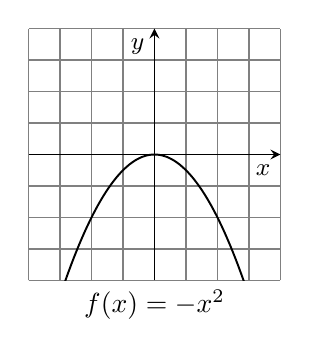
\begin{tikzpicture}[scale=0.800]
  % grid
  \draw[draw=black!50!white] (-2.000, -2.000) grid[step=0.5] (2.000, 2.000);
  % x-axis
  \draw[line width=0.6pt, ->, >=stealth] (-2.000, 0) -- (2.000, 0) node[below left] {\small$x$};
  % y-axis
  \draw[line width=0.6pt, ->, >=stealth] (0, -2.000) -- (0, 2.000) node[below left] {\small$y$};
  % function: f(x)=-x^{2}
  \begin{scope}[line width=0.7pt]
    \clip (-2.000, -2.000) rectangle (2.000, 2.000);
    \draw plot[smooth] coordinates
    {
      ( -2.000,  -4.000) ( -1.900,  -3.610) ( -1.800,  -3.240)
      ( -1.700,  -2.890) ( -1.600,  -2.560) ( -1.500,  -2.250)
      ( -1.400,  -1.960) ( -1.300,  -1.690) ( -1.200,  -1.440)
      ( -1.100,  -1.210) ( -1.000,  -1.000) ( -0.900,  -0.810)
      ( -0.800,  -0.640) ( -0.700,  -0.490) ( -0.600,  -0.360)
      ( -0.500,  -0.250) ( -0.400,  -0.160) ( -0.300,  -0.090)
      ( -0.200,  -0.040) ( -0.100,  -0.010) (  0.000,   0.000)
      (  0.100,  -0.010) (  0.200,  -0.040) (  0.300,  -0.090)
      (  0.400,  -0.160) (  0.500,  -0.250) (  0.600,  -0.360)
      (  0.700,  -0.490) (  0.800,  -0.640) (  0.900,  -0.810)
      (  1.000,  -1.000) (  1.100,  -1.210) (  1.200,  -1.440)
      (  1.300,  -1.690) (  1.400,  -1.960) (  1.500,  -2.250)
      (  1.600,  -2.560) (  1.700,  -2.890) (  1.800,  -3.240)
      (  1.900,  -3.610) (  2.000,  -4.000)
    };
  \end{scope}
  \node[below] at (0, -2) {$f(x)=-x^2$};
\end{tikzpicture}
%</OCTAVE>
%mypolyplot([-1 0 0], -2, 2, -2, 2, 0.1, 0.8)
\hfill
%<OCTAVE>
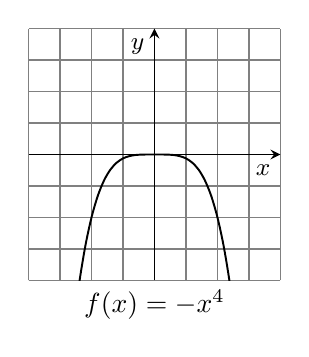
\begin{tikzpicture}[scale=0.800]
  % grid
  \draw[draw=black!50!white] (-2.000, -2.000) grid[step=0.5] (2.000, 2.000);
  % x-axis
  \draw[line width=0.6pt, ->, >=stealth] (-2.000, 0) -- (2.000, 0) node[below left] {\small$x$};
  % y-axis
  \draw[line width=0.6pt, ->, >=stealth] (0, -2.000) -- (0, 2.000) node[below left] {\small$y$};
  % function: f(x)=-x^{4}
  \begin{scope}[line width=0.7pt]
    \clip (-2.000, -2.000) rectangle (2.000, 2.000);
    \draw plot[smooth] coordinates
    {
      ( -2.000,  -5.000) ( -1.900,  -5.000) ( -1.800,  -5.000)
      ( -1.700,  -5.000) ( -1.600,  -5.000) ( -1.500,  -5.000)
      ( -1.400,  -3.842) ( -1.300,  -2.856) ( -1.200,  -2.074)
      ( -1.100,  -1.464) ( -1.000,  -1.000) ( -0.900,  -0.656)
      ( -0.800,  -0.410) ( -0.700,  -0.240) ( -0.600,  -0.130)
      ( -0.500,  -0.062) ( -0.400,  -0.026) ( -0.300,  -0.008)
      ( -0.200,  -0.002) ( -0.100,  -0.000) (  0.000,   0.000)
      (  0.100,  -0.000) (  0.200,  -0.002) (  0.300,  -0.008)
      (  0.400,  -0.026) (  0.500,  -0.062) (  0.600,  -0.130)
      (  0.700,  -0.240) (  0.800,  -0.410) (  0.900,  -0.656)
      (  1.000,  -1.000) (  1.100,  -1.464) (  1.200,  -2.074)
      (  1.300,  -2.856) (  1.400,  -3.842) (  1.500,  -5.000)
      (  1.600,  -5.000) (  1.700,  -5.000) (  1.800,  -5.000)
      (  1.900,  -5.000) (  2.000,  -5.000)
    };
  \end{scope}
  \node[below] at (0, -2) {$f(x)=-x^4$};
\end{tikzpicture}
%</OCTAVE>
%mypolyplot([-1 0 0 0 0], -2, 2, -2, 2, 0.1, 0.8)
\hfill
%<OCTAVE>
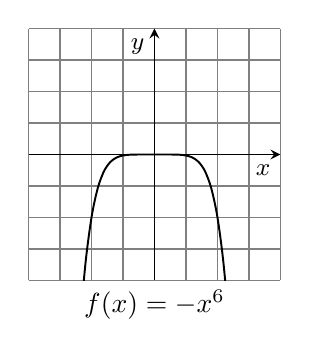
\begin{tikzpicture}[scale=0.800]
  % grid
  \draw[draw=black!50!white] (-2.000, -2.000) grid[step=0.5] (2.000, 2.000);
  % x-axis
  \draw[line width=0.6pt, ->, >=stealth] (-2.000, 0) -- (2.000, 0) node[below left] {\small$x$};
  % y-axis
  \draw[line width=0.6pt, ->, >=stealth] (0, -2.000) -- (0, 2.000) node[below left] {\small$y$};
  % function: f(x)=-x^{6}
  \begin{scope}[line width=0.7pt]
    \clip (-2.000, -2.000) rectangle (2.000, 2.000);
    \draw plot[smooth] coordinates
    {
      ( -2.000,  -5.000) ( -1.900,  -5.000) ( -1.800,  -5.000)
      ( -1.700,  -5.000) ( -1.600,  -5.000) ( -1.500,  -5.000)
      ( -1.400,  -5.000) ( -1.300,  -4.827) ( -1.200,  -2.986)
      ( -1.100,  -1.772) ( -1.000,  -1.000) ( -0.900,  -0.531)
      ( -0.800,  -0.262) ( -0.700,  -0.118) ( -0.600,  -0.047)
      ( -0.500,  -0.016) ( -0.400,  -0.004) ( -0.300,  -0.001)
      ( -0.200,  -0.000) ( -0.100,  -0.000) (  0.000,   0.000)
      (  0.100,  -0.000) (  0.200,  -0.000) (  0.300,  -0.001)
      (  0.400,  -0.004) (  0.500,  -0.016) (  0.600,  -0.047)
      (  0.700,  -0.118) (  0.800,  -0.262) (  0.900,  -0.531)
      (  1.000,  -1.000) (  1.100,  -1.772) (  1.200,  -2.986)
      (  1.300,  -4.827) (  1.400,  -5.000) (  1.500,  -5.000)
      (  1.600,  -5.000) (  1.700,  -5.000) (  1.800,  -5.000)
      (  1.900,  -5.000) (  2.000,  -5.000)
    };
  \end{scope}
  \node[below] at (0, -2) {$f(x)=-x^6$};
\end{tikzpicture}
%</OCTAVE>
%mypolyplot([-1 0 0 0 0 0 0], -2, 2, -2, 2, 0.1, 0.8)
\hfill
%<OCTAVE>
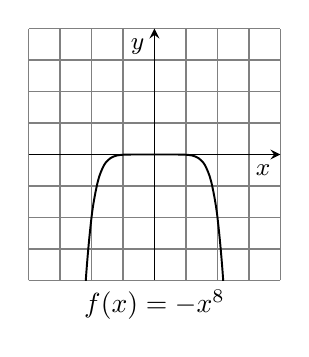
\begin{tikzpicture}[scale=0.800]
  % grid
  \draw[draw=black!50!white] (-2.000, -2.000) grid[step=0.5] (2.000, 2.000);
  % x-axis
  \draw[line width=0.6pt, ->, >=stealth] (-2.000, 0) -- (2.000, 0) node[below left] {\small$x$};
  % y-axis
  \draw[line width=0.6pt, ->, >=stealth] (0, -2.000) -- (0, 2.000) node[below left] {\small$y$};
  % function: f(x)=-x^{8}
  \begin{scope}[line width=0.7pt]
    \clip (-2.000, -2.000) rectangle (2.000, 2.000);
    \draw plot[smooth] coordinates
    {
      ( -2.000,  -5.000) ( -1.900,  -5.000) ( -1.800,  -5.000)
      ( -1.700,  -5.000) ( -1.600,  -5.000) ( -1.500,  -5.000)
      ( -1.400,  -5.000) ( -1.300,  -5.000) ( -1.200,  -4.300)
      ( -1.100,  -2.144) ( -1.000,  -1.000) ( -0.900,  -0.430)
      ( -0.800,  -0.168) ( -0.700,  -0.058) ( -0.600,  -0.017)
      ( -0.500,  -0.004) ( -0.400,  -0.001) ( -0.300,  -0.000)
      ( -0.200,  -0.000) ( -0.100,  -0.000) (  0.000,   0.000)
      (  0.100,  -0.000) (  0.200,  -0.000) (  0.300,  -0.000)
      (  0.400,  -0.001) (  0.500,  -0.004) (  0.600,  -0.017)
      (  0.700,  -0.058) (  0.800,  -0.168) (  0.900,  -0.430)
      (  1.000,  -1.000) (  1.100,  -2.144) (  1.200,  -4.300)
      (  1.300,  -5.000) (  1.400,  -5.000) (  1.500,  -5.000)
      (  1.600,  -5.000) (  1.700,  -5.000) (  1.800,  -5.000)
      (  1.900,  -5.000) (  2.000,  -5.000)
    };
  \end{scope}
  \node[below] at (0, -2) {$f(x)=-x^8$};
\end{tikzpicture}
%</OCTAVE>
%mypolyplot([-1 0 0 0 0 0 0 0 0], -2, 2, -2, 2, 0.1, 0.8)

% ------------------------------------------------------------------------------
\end{document}
% ------------------------------------------------------------------------------

